\documentclass[11pt]{article}

\usepackage{graphicx}
\usepackage{url}
\newcommand{\numpy}{{\tt numpy}}    % tt font for numpy
\topmargin -1in
\textheight 9in
\oddsidemargin -.25in
\evensidemargin -.25in
\textwidth 7in

\begin{document}

% https://moodle.up.pt/mod/assign/view.php?id=72723
\author{Miguel Sozinho Ramalho, UP201403027}
\date{March $6^{th}$, 2019}
\title{Algorithms for Bioinformatics: Project 2\\Definition of Python Class for Sequence Alignment}
\maketitle

% \medskip

\section{Introduction}
The current report describes a practical approach for extending the Python3 library developed in Project 1 to be capable of performing alignment on the defined biological sequences, namely local and global alignment, using the Needleman–Wunsch and Smith–Waterman algorithms, respectively. It is considered paramount that, in the case of multiple optimal solutions, all of them are discovered. The new version also contains relevant methods that can be used to better understand how the alignment works, such as visualisation for dot plots and other metrics, such as Hamming distance. Moreover, a large effort was made to allow for reusable, tested, documented and efficient code. Contextualising, this project belongs to the course of Algorithms in Bioinformatics.
% Contextualizar e descrever brevemente o problema.

\section{Implementation}
The main challenge of this project was the simple and correct implementation of the Dynamic Programming algorithms and also how to refactor the old module to achieve this goal. 

From the first project, only one new class was introduced: \textbf{Matrix}, this was an isolation of numerical matrices with the functionality required by the remaining algorithms and classes (and others used during the development), namely: sum, max, min, square, last, add\_val, mul\_val, apply, display, set\_col, \_\_len\_\_, \_\_setitem\_\_, \_\_getitem\_\_, \_\_iter\_\_, \_\_str\_\_ (this last one was particulary challenging as it was required for a smart pretty printing functionality). The precise goal of each function is described in the documentation of the class. 

In order to guarantee a good quality of the tool, it was required to write unit tests for all the developed methods (see Figure \ref{fig:coverageReport} for the 100\% coverage) and to document every implemented feature. 
% Descrição e estratégias de implementação - Discutir abordagens relevantes ao problema.

\begin{figure}[h!]
    \centering
    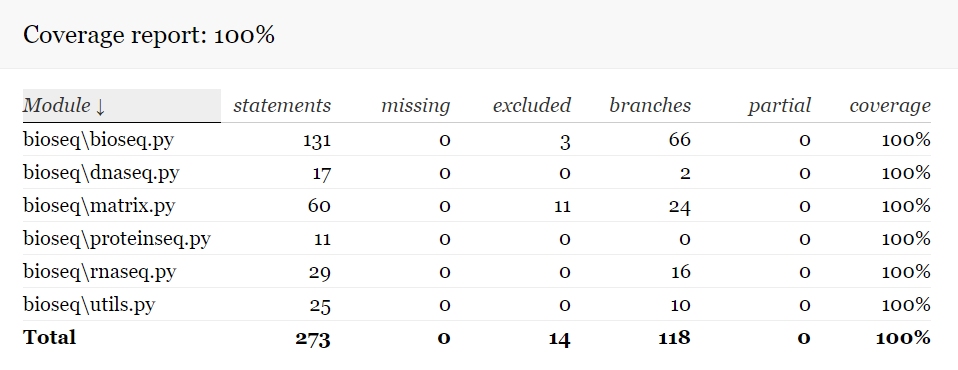
\includegraphics[width=0.65\textwidth]{coverageReport.png}
    \caption{Automatically generated test coverage report for the developed Python module}
    \label{fig:coverageReport}
\end{figure}

\section{Results}
All of the required functionality was implemented and also some others that were inspired by the work done in the practical lectures, namely:
\begin{itemize}
    \itemsep0em 
    \item hamming distance calculator (hamming\_distance)
    \item create a dotplot between two sequences (dot\_plot)
    \item display the dot\_plot in a plot if matplotlib is installed (display\_dot\_plot)
    \item score of aligning two sequences, given a gap and substitution matrix (score\_seq)
    \item affine gap score, using the gap penalty and the keep gap penalty (score\_affine\_gap)
    \item Needleman–Wunsch (global\_align\_multiple\_solutions)
    \item given two sequences and their global Score and Traceback matrices, return all the optimal alignments (recover\_global\_align\_multiple\_solutions)
    \item Smith–Waterman (local\_align\_multiple\_solutions)
    \item given two sequences and their local Score and Traceback matrices,     return all the local alignments (recover\_local\_align\_multiple\_solutions)
    \item for every combination return Score and Traceback matrices, global alignment (compare\_pairwise\_global\_align)
    \item for every combination return Score and Traceback matrices, local alignment (compare\_pairwise\_local\_align)
\end{itemize}

Some other interesting points:
\begin{itemize}
    \itemsep0em
    \item optimisation of the calculation of symmetric matrices
    \item the recovery algorithm is also very scalable as it is not recursive (as the original implementation) and takes a total of three very eloquent lines
    \item tests, documentation, code structure, Continuous Integration with  \url{https://travis-ci.com/} and push notifications of pipeline success with \url{https://www.pushbullet.com/} (see the \textit{pushbullet\_notify.py})
\end{itemize}


The documentation can be seen by opening the file \textit{docs/\_build/html/index.html} in an external browser or by typing \textbf{help(bioseq.moduleName)} on the Python console for the desired module. 

% Deve indicar que funcionalidades foram implementadas, se conseguiu implementar todas as funcionalidades pedidas e se implementou outras funcionalidades além das especificadas.

\section{Conclusions}
Looking back at all the progress made with this project, the author concludes there was a lot learned and also that most concepts became clearer when they had to be organised so meticulously, as in the current tool. It is his belief that the work produced is of sufficient quality to be used in future projects and also to be extended as more relevant bioinformatics and dynamic programming techniques are learned.
% Comentários e Conclusões.

\section{References}
\textit{(No paper references required and all other mentions like Python, FASTA, DNA, RNA, Aminoacid, OOP, Needleman–Wunsch, Smith–Waterman, Dynamic Programming and others are considered base knowledge prior to reading this document)}
%  (precisam ser explicitamente citadas no texto para saberem de onde o texto foi retirado/adaptado! Copiar é crime e poderá transformar-se em processo disciplinar, portanto evitem copiar textos e códigos. Se utilizarem figuras retiradas da web ou de livros ou de artigos etc, é necessário colocar uma referência explícita e clara. Por favor tenham atenção aos erros ortográficos.


\end{document}
\grid
\grid